\documentclass{beamer}
\usetheme{Warsaw}  %% Themenwahl

\usepackage[utf8]{inputenc}
\usepackage[ngerman]{babel}
\usepackage{ngerman}
\usepackage{wrapfig}
\usepackage{multicol}
\usepackage{color}
\usepackage{multicol}

\graphicspath{{../}}
%\pdfimageresolution=300
 
\title[Analyse von SHA256 mit Hilfe von CryptoMiniSat]{Kolloquium zur Masterarbeit:\newline Analyse von SHA256 mit Hilfe von CryptoMiniSat}
\author{Lars Schmertmann}
\date{\vspace*{-1cm}\newline 14. Juni 2017\newline\newline Begutachtung durch:\newline Prof. Dr. Rolf Drechsler und Dr.-Ing. Olaf Bergmann\newline \newline Betreuung durch die AG Rechnerarchitektur:\newline Dr. Stephan Eggersglüß und Dr. Daniel Große}
 
\begin{document}
\maketitle
%\setcounter{tocdepth}{3}
%\frame{\tableofcontents}
%\frame{\tableofcontents[currentsection]}

\author{Lars Schmertmann}

\frame{ \begin{multicols}{2} \tableofcontents \end{multicols} }

\section{Einleitung}
  \subsection{Motivation}
    \begin{frame}{Motivation}
      \begin{itemize}
        \setlength{\itemsep}{12pt}
        \item Urbildresistenz vs. SAT-Solver
        \item Flexibel, beliebige Vorgaben möglich
        \begin{itemize}
          \item Bitcoin sehr stark eingeschränkt - kleiner Lösungsraum
        \end{itemize}
        \item Andere Masterarbeiten konzentrieren sich auf SAT-Solver
        \item Masterarbeit zum Thema SHA1/SAT-Solver
        \begin{itemize}
          \item Universität Oslo - Vegard Nossum - November 2012
        \end{itemize}
        \item GitHub-Projekt von Martin Maurer: SHA256
        \item GitHub-Projekt von Jonathan Heusser: SatCoin - (CBMC)
      \end{itemize}
    \end{frame}
  \subsection{Hasheigenschaften}
    \begin{frame}{Hasheigenschaften}
      Ein guter kryptographischer Hash ist:\\
      ~\\
      \begin{itemize}
        \setlength{\itemsep}{20pt}
        \item Kollisionsresistent:
        \begin{itemize}
          \item schwer, $ x \neq y $ zu finden mit $ h(x) = h(y) $
        \end{itemize}
        \item Urbildresistent:
        \begin{itemize}
          \item schwer, zu einem $ a $ ein $ y $ zu finden mit $ a = h(y) $
        \end{itemize}
      \end{itemize}
      ~\\
      Gelingt es die Urbildresistenz zu umgehen,\\
      ist die Kollisionsresistenz ebenfalls umgangen.
    \end{frame}
\subsection{SHA256}
    \begin{frame}{SHA256 / Eckdaten}
      \begin{columns}[T]
        \column{.48\textwidth}
        \begin{itemize}
          \item Nachfolger von SHA-1\\
          \item Standardisierung durch\newline das NIST in 2001\\
          \item Arbeitet in 512 Bit Blöcken\\
          \item Erzeugt einen 256 Bit Hash\\
          \item Besteht aus:\\
          \begin{itemize}
            \item Padding\\
            \item Konstanten\\
            \item Erweiterung\\
            \item Berechnung
          \end{itemize}
        \end{itemize}
        \column{.52\textwidth}
        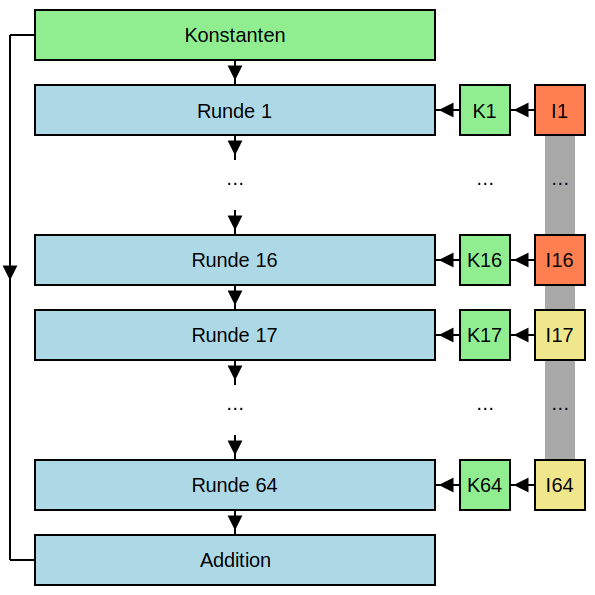
\includegraphics[scale=0.25]{sha256single}
      \end{columns} 
    \end{frame}
    \begin{frame}{SHA256 / Padding}
      Auffüllen der Eingabe auf ein Vielfaches von 512 Bit.\\
      ~\\
      Allgemeines Padding:\\
      ~\\
      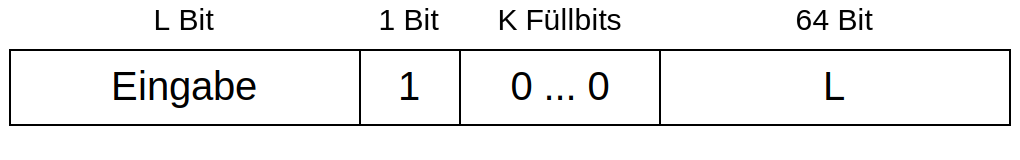
\includegraphics[width=300pt]{padding}\\
    \end{frame}
    \begin{frame}{SHA256 / Funktionen}
      \begin{itemize}
      \setlength{\itemsep}{20pt}
      \item Erweiterung
        \begin{itemize}
          \setlength{\itemsep}{10pt}
          \item $ SSIG0(x) = ROTR^{7}(x)~XOR~ROTR^{18}(x)~XOR~SHR^{3}(x) $
          \item $ SSIG1(x) = ROTR^{17}(x)~XOR~ROTR^{19}(x)~XOR~SHR^{10}(x) $
        \end{itemize}
      \item Berechnung
        \begin{itemize}
          \setlength{\itemsep}{10pt}
          \item $ CH( x, y, z) = (x~AND~y)~XOR~( (NOT~x)~AND~z) $
          \item $ MAJ( x, y, z) = (x~AND~y)~XOR~(x~AND~z)~XOR~(y~AND~z) $
          \item $ BSIG0(x) = ROTR^{2}(x)~XOR~ROTR^{13}(x)~XOR~ROTR^{22}(x) $
          \item $ BSIG1(x) = ROTR^{6}(x)~XOR~ROTR^{11}(x)~XOR~ROTR^{25}(x) $
        \end{itemize}
      \end{itemize}
    \end{frame}
    \begin{frame}{SHA256 / Erweiterung}
      Jeder Block der Länge 512 Bit wird auf 2048 Bit erweitert.\\
      ~\\
      Die zusätzlichen Bits werden wie folgt generiert:\\
      ~\\
      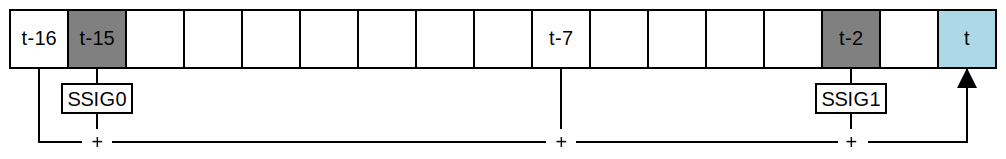
\includegraphics[width=300pt]{extend}
    \end{frame}
    \begin{frame}{SHA256 / Berechnung}
      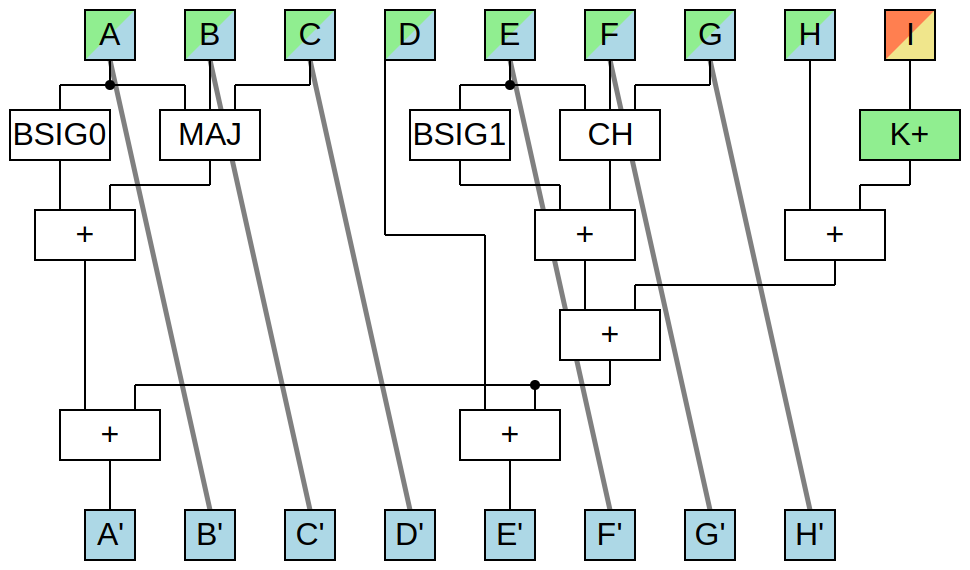
\includegraphics[width=300pt]{sha256core}
    \end{frame}
  \subsection{Bitcoin}
    \begin{frame}
      \frametitle{Bitcoin / Aufgabe}
      Aufbau eines Bitcoinblocks:
      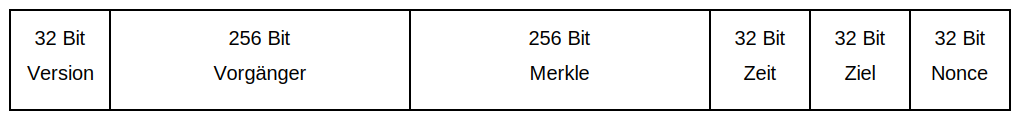
\includegraphics[width=300pt]{bitcoinblock}\\
      ~\\
      Aufgabe:\\
      Finde eine Nonce, so dass SHA256(SHA256(Block))\\
      kleiner als das aktuelle Ziel ist.\\
      ~\\
      Das bedeutet aktuell:\\
      Der Hashwert muss 67 führende Nullen haben.
    \end{frame}
    \begin{frame}{Bitcoin / Padding}
      Eingabe für die erste Hashberechnung:
      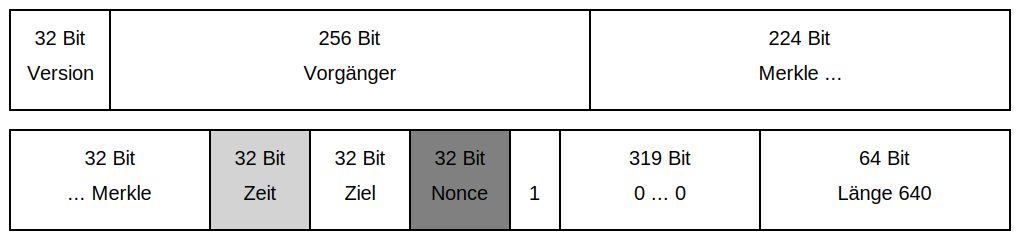
\includegraphics[width=300pt]{blockpadding}\\
      ~\\
      Eingabe für die zweite Hashberechnung:
      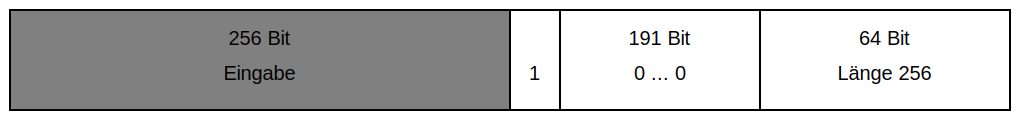
\includegraphics[width=300pt]{blockpadding2}\\
  \end{frame}
\section{Umsetzung}
  \begin{frame}{}
    \begin{center}
      \Huge Umsetzung
    \end{center}
  \end{frame}
  \subsection{CryptoMiniSat / Konjunktive Normalform}
    \begin{frame}{Sat-Solver}
      \begin{itemize}
        \setlength{\itemsep}{12pt}
        \item Versucht zu ermitteln, ob eine aussagenlogische Formel erfüllbar ist
        \item Falls erfüllbar, liefert der SAT-Solver ein Beispiel
        \item Lösbar in exponentieller Zeit bezüglich der Anzahl Variablen
        \begin{itemize}
          \item NP vollständig
        \end{itemize}
        \item Enthält u.a. Heuristiken und Lernverfahren
        \begin{itemize}
         \item Generiert Wissen
        \end{itemize}
        \item Transformation von SHA256 in ein Erfüllbarkeitsproblem
        \begin{itemize}
         \item In diesem Fall die konjunktive Normalform
        \end{itemize}
      \end{itemize}
    \end{frame}
    \begin{frame}{Konjunktive Normalform}
      \begin{itemize}
        \setlength{\itemsep}{16pt}
        \item Eine Formel der Aussagenlogik ist in konjunktiver Normalform, wenn sie eine Konjunktion von Disjunktionstermen ist
        \item Literal: nichtnegierte oder negierte Variable
        \item Klausel: ein Disjunktionsterm
        \item Eine Formel in KNF hat also die Form: \newline \newline $ \bigwedge\limits_{i} \bigvee\limits_{j} (\neg)x_{ij} $
        \item Beispiel: $ (\neg a \vee \neg b \vee \neg c) \wedge (\neg a \vee b \vee c) $
      \end{itemize}
    \end{frame}
    \begin{frame}{Espresso}
      Heuristic Logic Minimizer der Berkeley Universität von 1989\\
      ~\\
      Am Beispiel von AND:\\
      ~\\
      \begin{tabular}{ccc|cp{1cm}ccc|cp{1cm}l}
        a & b & r & c & & a & b & r & c\\
        \cline{1-4}\cline{6-9}
        1 & 1 & 0 & 0 & & 1 & 1 & 0 & 0 & & $ (\neg a \vee \neg b \vee c) $\\
        1 & 0 & 1 & 0 & & X & 0 & 1 & 0 & & $ (b \vee \neg c) $\\
        0 & 1 & 1 & 0 & & 0 & X & 1 & 0 & & $ (a \vee \neg c) $\\
        0 & 0 & 1 & 0 \\
        \cline{1-4}
        1 & 1 & 1 & 1 \\
        1 & 0 & 0 & 1 \\
        0 & 1 & 0 & 1 \\
        0 & 0 & 0 & 1 \\
      \end{tabular}
    \end{frame}
    \begin{frame}{XOR}
      Die Klauselmenge für ein XOR wächst exponentiell. Beispiel:\\
      ~\\
      $n = 2$:~~~~$ a \Leftrightarrow b \veebar c$\\
      ~\\
      4 Klauseln mit jeweils 3 Literalen
      ~\\
      $ (\neg a \vee \neg b \vee \neg c) \wedge (\neg a \vee b \vee c) \wedge (a \vee \neg b \vee c) \wedge (a \vee b \vee \neg c) $\\
      ~\\
      Allgemein: $ 2^{n} $ Klauseln mit jeweils $ n + 1 $ Literalen\\
      ~\\
      CryptoMiniSat akzeptiert auch XOR-Klauseln: $ (\neg a \veebar b \veebar c)$\\
    \end{frame}
  \subsection{Padding}
    \begin{frame}{Padding}
      Mögliche Lösung für SAT-Berechnung\\
      \begin{itemize}
       \item Länge von 55 Byte vorgeben:
      \end{itemize}
      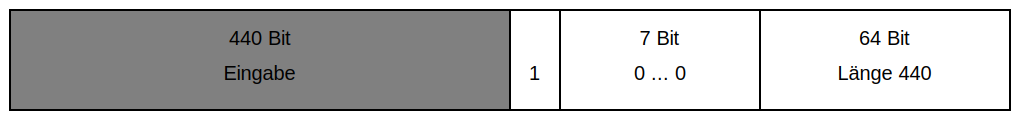
\includegraphics[width=300pt]{padding-allgemein}
    \end{frame}
  \subsection{Funktionen}
    \begin{frame}{CH - Choose}
      $ CH( x, y, z) = (x~AND~y)~XOR~( (NOT~x)~AND~z) $\\
      ~\\
      $ c \Leftrightarrow (x \wedge y) \veebar ( \neg x \wedge z) $\\
      ~\\
      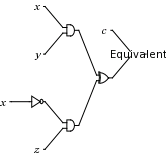
\includegraphics[scale=0.5]{ch.png}\\
      ~\\
      $ (\neg c \vee \neg x \vee y) \wedge (\neg c \vee x \vee z) \wedge (c \vee \neg x \vee \neg y) \wedge (c \vee x \vee \neg z) $
    \end{frame}
    \begin{frame}{MAJ - Majority}
      $ MAJ( x, y, z) = (x~AND~y)~XOR~(x~AND~z)~XOR~(y~AND~z) $\\
      ~\\
      $ m \Leftrightarrow (x \wedge y) \veebar (x \wedge z) \veebar (y \wedge z) $\\
      ~\\
      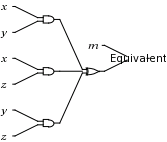
\includegraphics[scale=0.5]{maj.png}\\
      ~\\
      $ (\neg m \vee x \vee y) \wedge  (\neg m \vee x \vee z) \wedge (\neg m \vee y \vee z) \wedge $\\
      $ (m \vee \neg x \vee \neg y) \wedge (m \vee \neg x \vee \neg z) \wedge (m \vee \neg y \vee \neg z) $
      \end{frame}
    \begin{frame}{*SIG* - Small/Big Sigma}
      $ *SIG*(a, b, c) = a~XOR~b~XOR~c $\\
      ~\\
      $ s \Leftrightarrow a \veebar b \veebar c $\\
      ~\\      
      \begin{columns}[C]
        \column{.4\textwidth}
        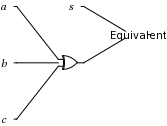
\includegraphics[scale=0.5]{sig.png}
        \column{.5\textwidth}
        $ \Rightarrow (\neg s \veebar a \veebar b \veebar c) $
      \end{columns}
      ~\\
      ~\\
      $ (\neg a \vee \neg b \vee \neg c \vee s) \wedge (\neg a \vee \neg b \vee c \vee \neg s) \wedge (\neg a \vee b \vee \neg c \vee \neg s) \wedge$\\
      $ (\neg a \vee b \vee c \vee s) \wedge (a \vee \neg b \vee \neg c \vee \neg s) \wedge (a \vee \neg b \vee c \vee s) \wedge $\\
      $ (a \vee b \vee \neg c \vee s) \wedge (a \vee b \vee c \vee \neg s) $
    \end{frame}
    \begin{frame}{Carry-Riple-Addierer}
      32 Bit Addierer : 1 Halbaddierer + 30 Volladdierer + 1 Mod2-Add.\\
      ~\\
      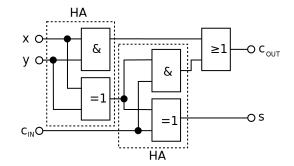
\includegraphics[scale=0.5]{volladdierer}\\
      $ (c_{out} \vee \neg x \vee \neg y) \wedge (\neg c_{out} \vee x \vee y) \wedge (c_{out} \vee \neg x \vee \neg c_{in}) \wedge $\\
      $ (c_{out} \vee \neg y \vee \neg c_{in}) \wedge (\neg c_{out} \vee x \vee c_{in}) \wedge (\neg c_{out} \vee y \vee c_{in}) $\\
      ~\\
      $ (\neg s \veebar x \veebar y \veebar c_{in})$\\
    \end{frame}
  \subsection{Komposition}
  \begin{frame}{Modulhierarchie}
     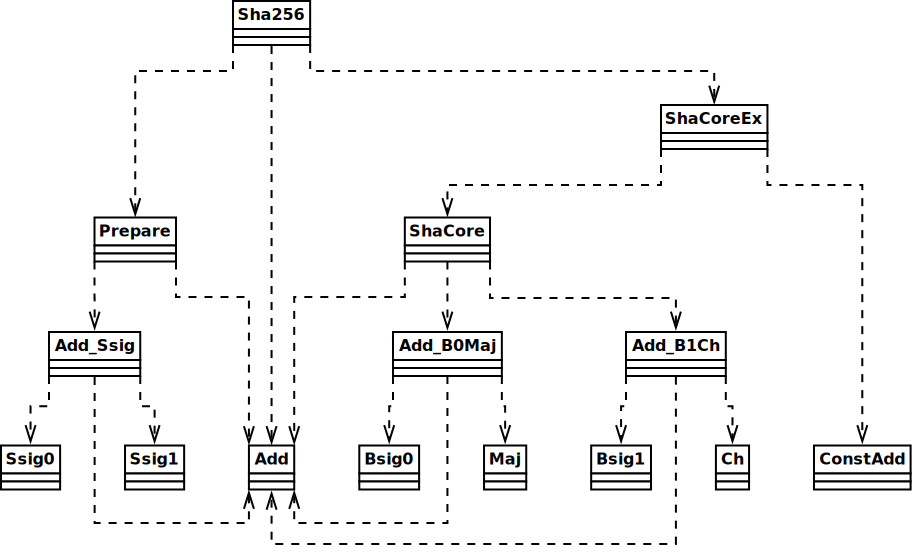
\includegraphics[scale=0.2]{module}
  \end{frame}
  \begin{frame}{Module mit Rekonvergenzen}
     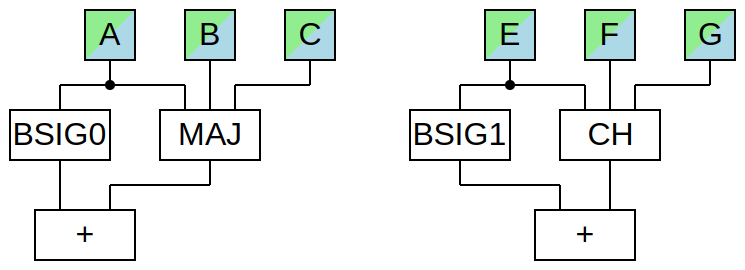
\includegraphics[scale=0.4]{sha256coreM}
  \end{frame}  
  \begin{frame}{Vergleich mit CBMC und Martin Maurer}
    \begin{multicols}{2}
      \begin{itemize}
        \setlength{\itemsep}{20pt}
	\item Eigenbau
	\begin{itemize}
	  \item $ \sim $ 50.000 Variablen
	  \item $ \sim $ 250.000 Klauseln
	  \item $ \sim $ 150.000 Klauseln (XOR)
	\end{itemize}
	\item CBMC
	\begin{itemize}
	  \item $ \sim $ 70.000 Variablen
	  \item $ \sim $ 350.000 Klauseln
	  \item keine XOR-Unterstützung
	\end{itemize}
	\item Martin Maurer - Espresso
	\begin{itemize}
	  \item $ \sim $ 60.000 Variablen
	  \item $ \sim $ 660.000 Klauseln
	  \item $ \sim $ 590.000 Klauseln (XOR)
	\end{itemize}
	\item Martin Maurer - Tseitin
	\begin{itemize}
	  \item $ \sim $ 130.000 Variablen
	  \item $ \sim $ 450.000 Klauseln
	  \item $ \sim $ 260.000 Klauseln (XOR)
	\end{itemize}
      \end{itemize}
    \end{multicols}
  \end{frame}

\section{Analyse}
  \begin{frame}{}
    \begin{center}
      \Huge Analyse
    \end{center}
  \end{frame}
  \subsection{Lösungsversuche}
    \begin{frame}{Lösungsversuche}
      \begin{itemize}
        \setlength{\itemsep}{20pt}
        \item Eingabe: "`Das ist eine Eingabe aus der ein Hash erstellt wird."'
        \item Hash:\newline
              27931f0e7e53670ddbec1a1ce23e21b4\newline
              663c63c0d17117ee1a934bc0c294dbe9
        \item Iterative Lösungsversuche - Vorgaben als Annahmen
        \item Bei jedem Lösungsversuch ein Bit mehr vorgeben
        \item Nach einer erfolgreichen Lösung: Konfliktklauseln exportieren
      \end{itemize}
    \end{frame}
  \subsection{Analyse der Konfliktklauseln}
    \begin{frame}{Analyse der Konfliktklauseln}
      \begin{enumerate}
        \setlength{\itemsep}{20pt}
        \item Entfernen schon bekannter Klauseln
        \pause
        \item Identifizierung und Normalisierung modulspezifischer Klauseln
        \pause
        \item Bewertung der modulübergreifenden Klauseln:
        \begin{itemize}
          \item SHA256 als ungerichter Graph mit ca. 1000 Knoten
          \item Berechnung der Distanz der Knoten zueinander mit Dijkstra
          \item Klauselbewertung ergibt sich durch: max\_dist - module + 1
          \item Der Wert beschreibt, wie viele Knoten übersprungen werden
        \end{itemize}
        \pause
        \item Prüfen auf kürzere/längere Klauseln
      \end{enumerate}
    \end{frame}
  \subsection{Verallgemeinerung von Klauseln}
    \begin{frame}{Weitere Konfliktklauseln testen}
      \begin{itemize}
        \setlength{\itemsep}{20pt}
        \item "`Wertvolle"' Klauseln übertragen auf:
        \begin{itemize}
          \item Vorhergehende oder Nachfolgende Runden
          \item Vorhergehende oder Nachfolgende Bits
        \end{itemize}
        \item Erzeugte Klauseln auf Gültigkeit überprüfen
        \item Bei vielen Klauseln sehr erfolgreich
      \end{itemize}
    \end{frame}
  \subsection{Erhaltene Klauseln}
    \begin{frame}{Erhaltene Klauseln}
      \begin{itemize}
        \item Die meisten Klauseln kommen aus den Addierern: Lassen sich durch Carry-Look-Ahead-Addiere unterschiedlicher Bitbreite in mehreren Ebenen beschreiben
        \pause
        \item Klauseln über Distanz:\newline
        \begin{tabular}{rrrr}
          Distanz & Gesamt & Redundant & Verbleibend\\
          \hline
                1 &    840 &       114 &   726\\
                2 &   5337 &      1475 &  3862\\
                3 &  11139 &      3295 &  7844\\
                4 &  10002 &      3324 &  6678\\
                5 &   2403 &       207 &  2196\\
          \hline
                  &        &           & 21306
        \end{tabular}
      \end{itemize}
    \end{frame}

\section{Ergebnisse}
  \begin{frame}{}
    \begin{center}
      \Huge Ergebnisse
    \end{center}
  \end{frame}
  \subsection{Bewertung der erhaltenen Klauseln}
    \begin{frame}{Bewertung der erhaltene Klauseln}
      \begin{tabular}{l|rr|rr}
	Klauselmenge    & \multicolumn{2}{c|}{mit XOR} & \multicolumn{2}{c}{ohne XOR} \\
	\hline
	Original        &  194:27 & 100\% &   169:24 & 100\% \\
	\hline
	Modulspezifisch &   91:28 &  47\% &    69:07 &  41\% \\
	Distanz         &  155:31 &  80\% &   141:34 &  84\% \\
	Addierer        &  410:59 & 211\% &   491:53 & 290\% \\
	Zusätzlich      &  205:09 & 105\% &   100:41 &  59\% \\
	\hline
	Kombiniert      &  244:36 & 126\% &   136:37 &  81\%    
      \end{tabular}
    \end{frame}
  \subsection{Vergleich mit CBMC und Martin Maurer}
    \begin{frame}{Vergleich mit CBMC und Martin Maurer}
      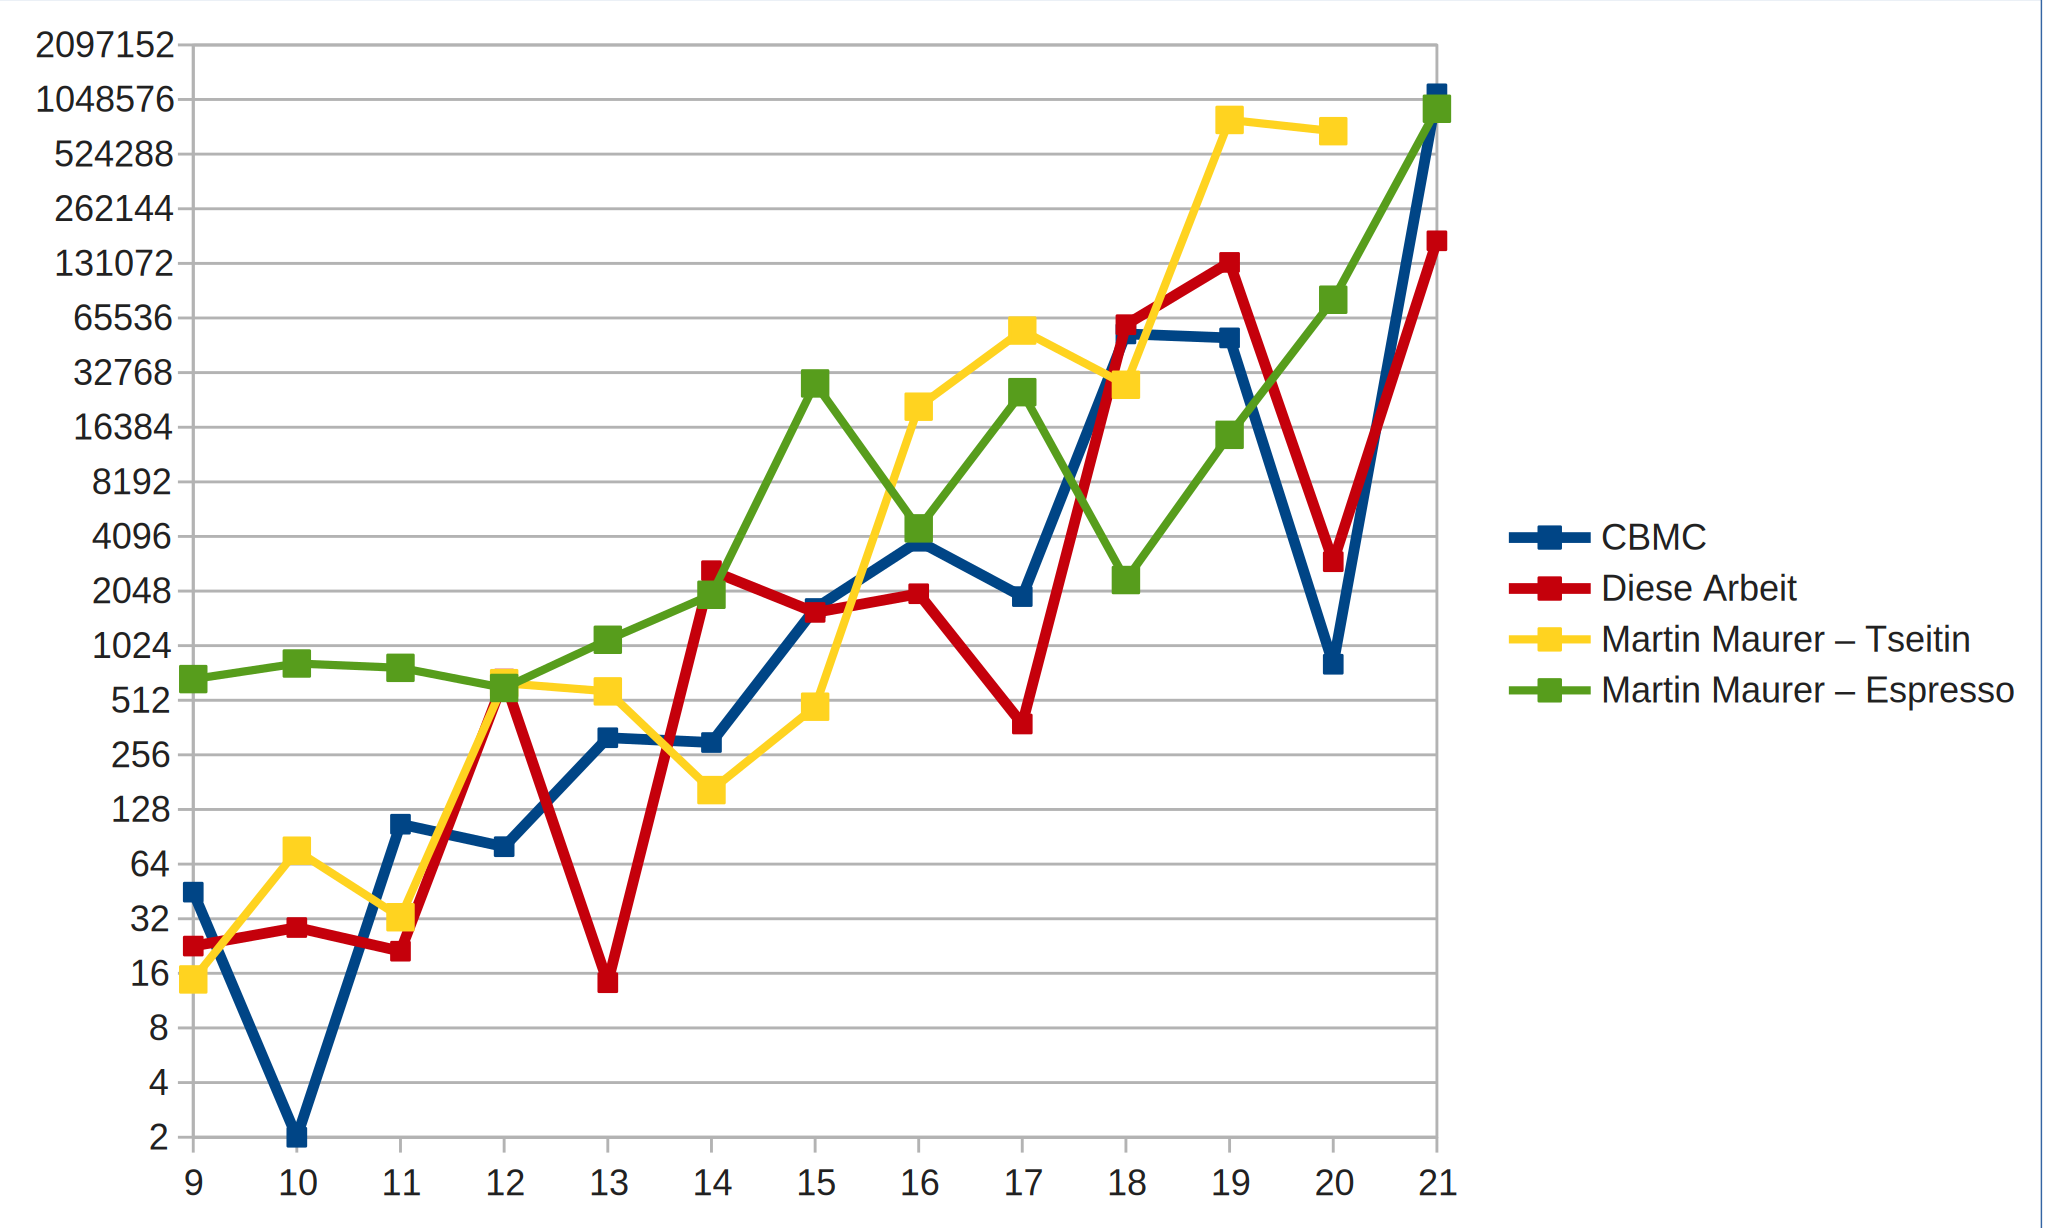
\includegraphics[scale=0.4]{eval_final}
    \end{frame}
  \subsection{Bedeutung für SHA256}
    \begin{frame}{Initialwertberechnung}
      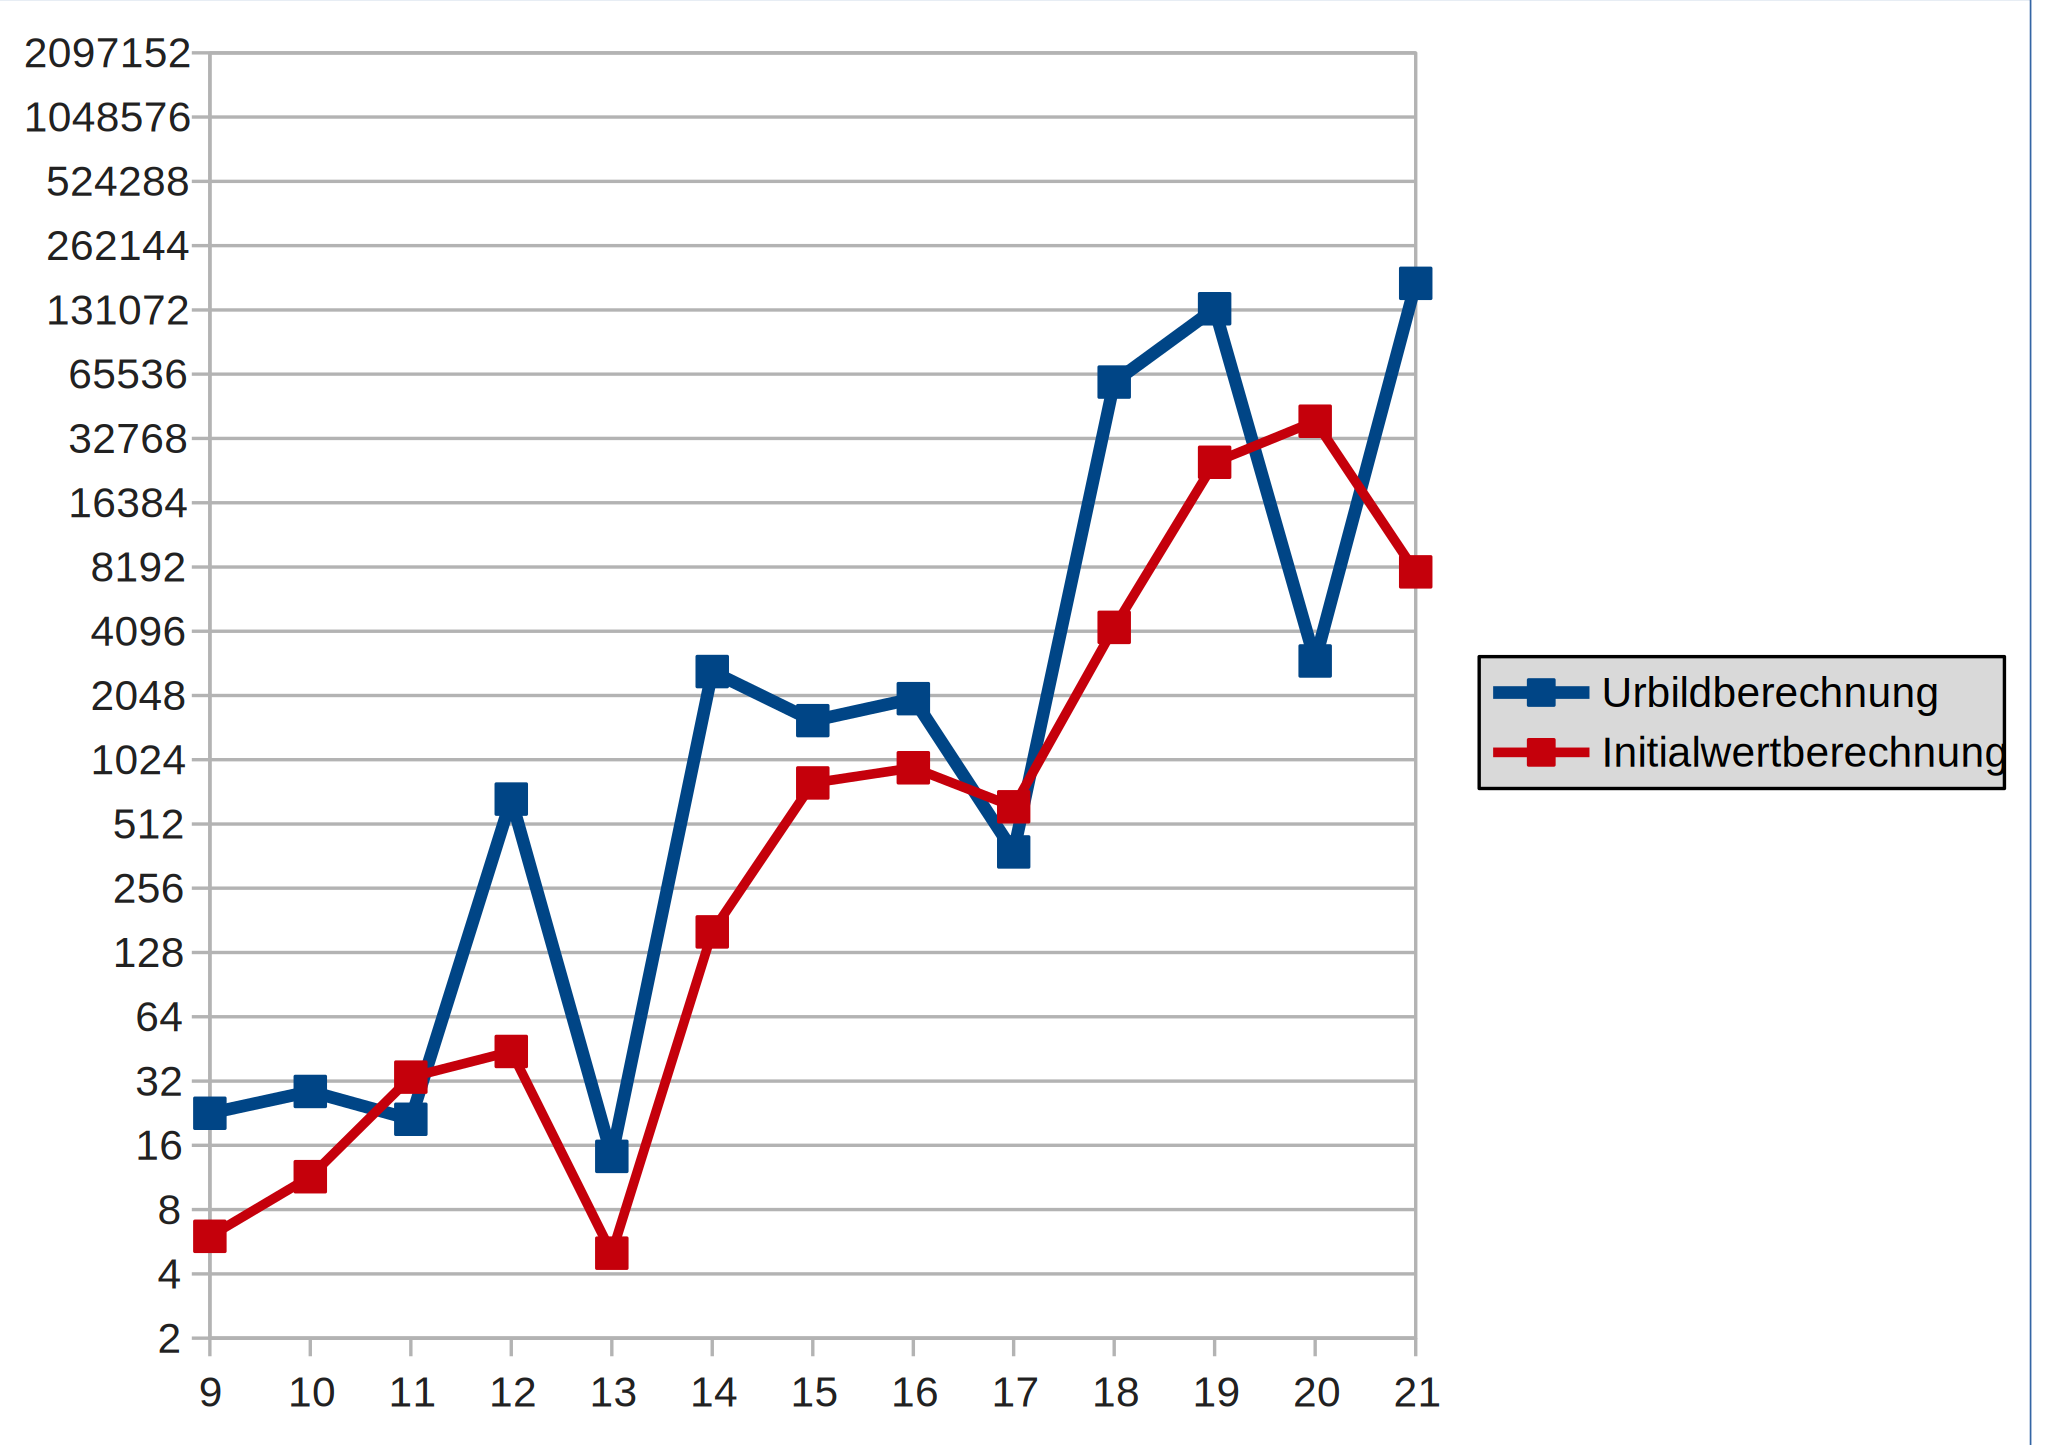
\includegraphics[scale=0.4]{eval_initial}
    \end{frame}
    \begin{frame}{Kollisionsberechnung}
      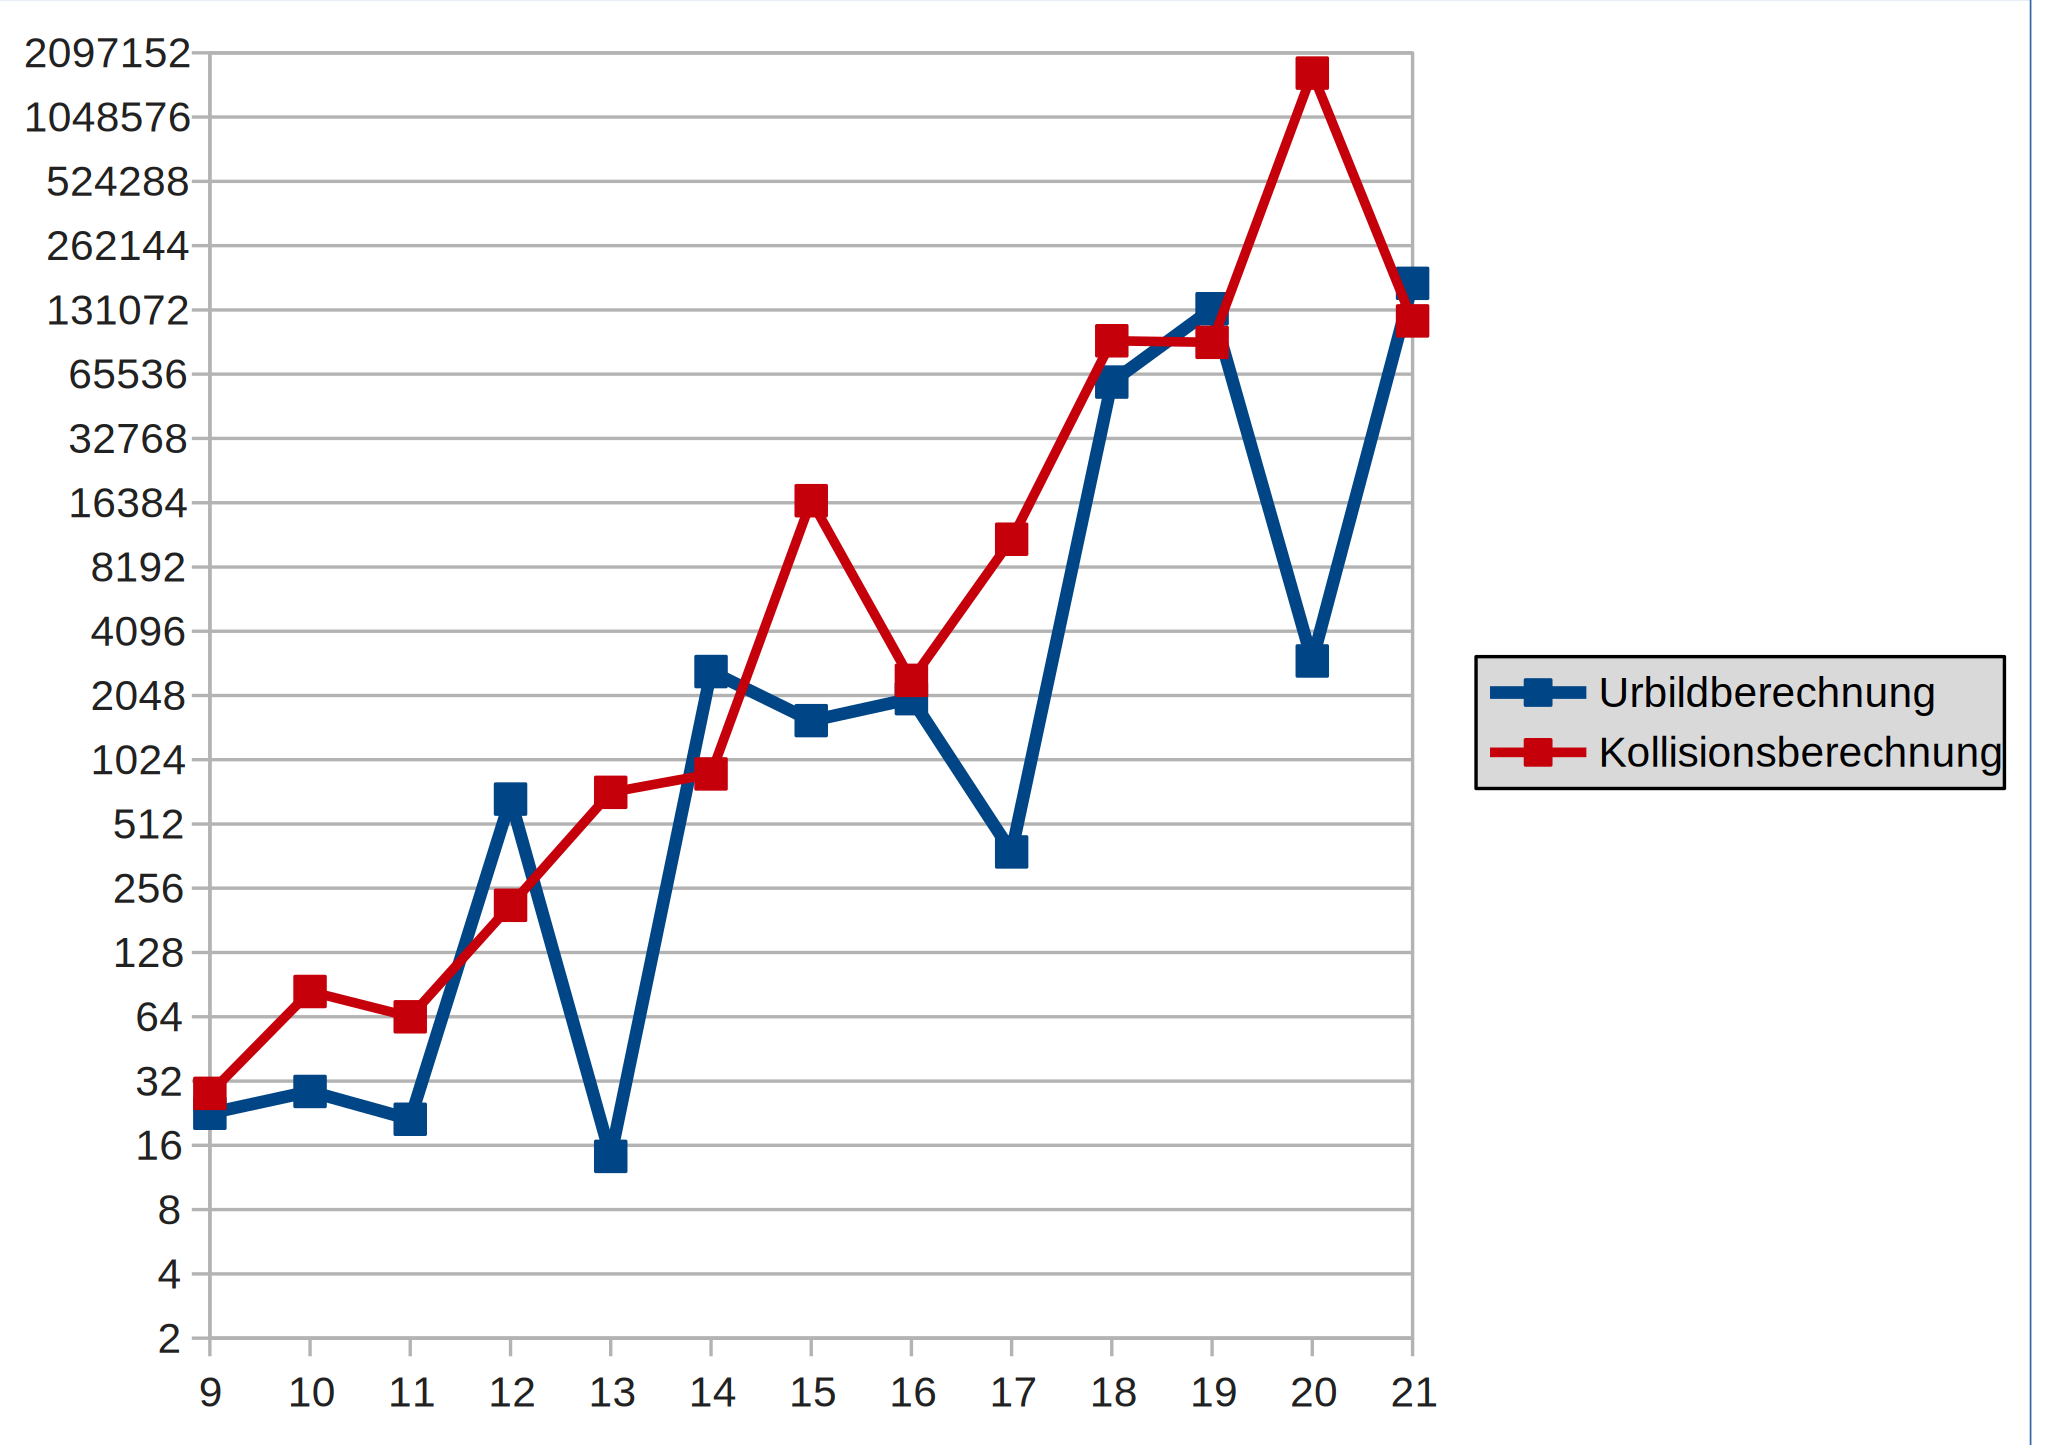
\includegraphics[scale=0.4]{eval_kollision}
    \end{frame}
  \subsection{Bedeutung für Bitcoin}
    \begin{frame}{Bedeutung für Bitcoin}
      \begin{tabular}{rr|rr}
        Geforderte Nullen & Dauer in Minuten & Erhaltene Nullen \\
        \hline
         9 &  0:43 &  9 \\
        10 &  1:55 & 10 \\
        11 &  8:32 & 11 \\
        12 &  5:29 & 14 \\
        13 & 10:39 & 16
      \end{tabular}
    \end{frame}

\begin{frame}{}
  \begin{center}
    \begin{LARGE}
      Vielen Dank für\\
      eure Aufmerksamkeit\\
      ~\\
      
\includegraphics[scale=0.2]{smilie.png}
    \end{LARGE}
  \end{center}
\end{frame}

\begin{frame}{Fragen}
  \begin{center}
    \begin{LARGE}
      \begin{tabular}{ccccc}
         & \textbf{?} & \textbf{?} & \textbf{?} & \\
        \textbf{?} & \textbf{?} &  & \textbf{?} & \textbf{?}\\
         &  &  & \textbf{?} & \textbf{?}\\
         &  & \textbf{?} & \textbf{?} & \\
         & \textbf{?} & \textbf{?} &  & \\
         &  &  &  & \\
         & \textbf{?} & \textbf{?} &  & \\
         & \textbf{?} & \textbf{?} &  & 
      \end{tabular}
    \end{LARGE}
  \end{center}
\end{frame}

\end{document}